\documentclass[tikz,border=8pt]{standalone}
% Shared look for every TikZ diagram. Load with \input{../../tools/tikz-style.tex}
\usepackage[sfdefault]{roboto}
\usetikzlibrary{arrows.meta, positioning, shapes.geometric, calc, fit, backgrounds}
\definecolor{cblue}{HTML}{4C78A8}
\definecolor{corange}{HTML}{F58518}
\definecolor{cgreen}{HTML}{54A24B}
\definecolor{cred}{HTML}{E45756}
\definecolor{cpurple}{HTML}{B279A2}
\definecolor{cgrey}{HTML}{6B6B6B}
\tikzset{
  every picture/.style={font=\sffamily, line width=1.2pt},
  box/.style={draw=#1, fill=#1!12, rounded corners=4pt, align=center, inner sep=7pt, minimum height=1.1cm},
  box/.default=cgrey,
  arrow/.style={-{Stealth[length=3mm]}, draw=cgrey, line width=1.4pt},
  title/.style={font=\sffamily\bfseries\Large},
  note/.style={font=\sffamily\small, text=cgrey, align=center},
}
\AtBeginDocument{\hyphenpenalty=10000 \exhyphenpenalty=10000}

% The same car, 1.0 s into the run, measured at two points. Rear axle (1.980, 0.737), heading -10.74 deg; front axle
% 2.5 m ahead at (4.436, 0.271). On the straight the lateral errors are 0.737 m and 0.271 m:
% 0.737 + 2.5 x sin(-10.74 deg) = 0.737 - 0.466 = 0.271.
\begin{document}
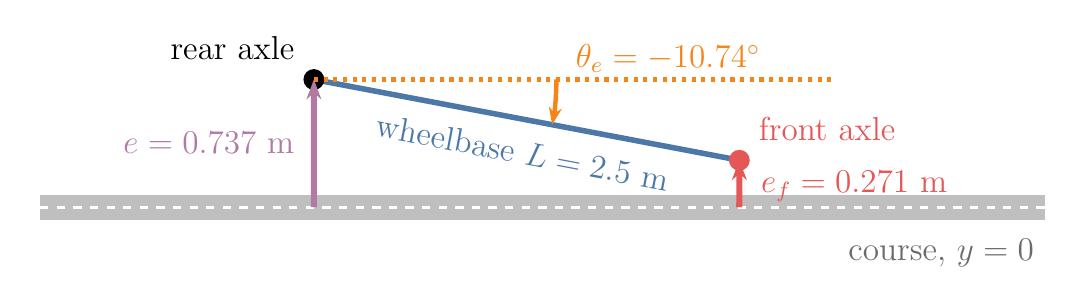
\begin{tikzpicture}[scale=2.2, every node/.append style={font=\large}]
  % the course's first straight, y = 0
  \draw[black!25, line width=9pt] (0.4,0) -- (6.2,0);
  \draw[white, dashed, line width=1pt] (0.4,0) -- (6.2,0);
  \node[cgrey, anchor=north east] at (6.2,-0.12) {course, $y = 0$};
  % axle points and the centre line between them
  \coordinate (R) at (1.980,0.737);
  \coordinate (F) at (4.436,0.271);
  \draw[cblue, line width=2pt] (R) -- (F);
  \fill[black] (R) circle (0.06);
  \fill[cred] (F) circle (0.06);
  \node[anchor=south east] at ($(R)+(-0.05,0.05)$) {rear axle};
  \node[cred, anchor=south west] at ($(F)+(0.05,0.05)$) {front axle};
  % lateral errors, straight down to the course
  \draw[-{Stealth[length=2.5mm]}, cpurple, line width=2.2pt] (1.980,0) -- (R);
  \node[cpurple, anchor=east] at (1.93,0.37) {$e = 0.737$ m};
  \draw[-{Stealth[length=2.5mm]}, cred, line width=2.2pt] (4.436,0) -- (F);
  \node[cred, anchor=west] at (4.5,0.12) {$e_f = 0.271$ m};
  % wheelbase label along the car
  \node[cblue, anchor=north, rotate=-10.74] at ($(R)!0.5!(F)+(0,-0.06)$) {wheelbase $L = 2.5$ m};
  % heading error at the rear axle: course direction (dotted) to the heading
  \draw[corange, dotted, line width=1.5pt] (R) -- ++(0:3.0);
  \draw[-{Stealth[length=2.2mm]}, corange, line width=1.6pt] ($(R)+(0:1.4)$) arc (0:-10.74:1.4);
  \node[corange, anchor=west] at ($(R)+(0:1.45)+(0,0.12)$) {$\theta_e = -10.74^\circ$};
\end{tikzpicture}
\end{document}
